\textbf{COLUNI 2020 -- Questão 35}\par\medskip Analise os documentos abaixo.

\textbf{Documento I}

% COLUNI-AUTO-FIGURES-BEGIN
\begin{figure}[htbp]
\centering
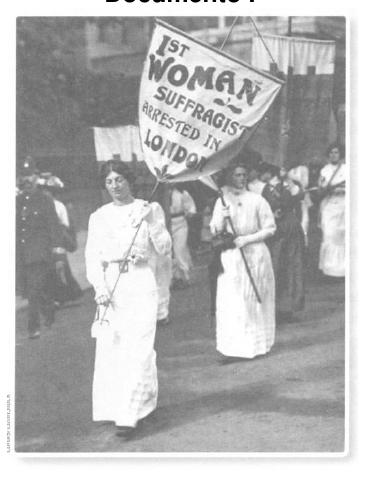
\includegraphics[width=0.95\linewidth]{static/simulados/coluni/figuras/2020/questao-35/figura-1.png}
\end{figure}
% COLUNI-AUTO-FIGURES-END

Londres, 1905. Passeata comemorando a primeira eleição com votos femininos. No cartaz está escrito “Primeira mulher sufragista presa em Londres” (tradução livre).

VICENTINO, Cláudio. \textbf{Projeto Radix}: História, 9º ano. São Paulo: Scipione, 2009, p. 15.

\textbf{Documento II}

% COLUNI-AUTO-FIGURES-BEGIN
\begin{figure}[htbp]
\centering
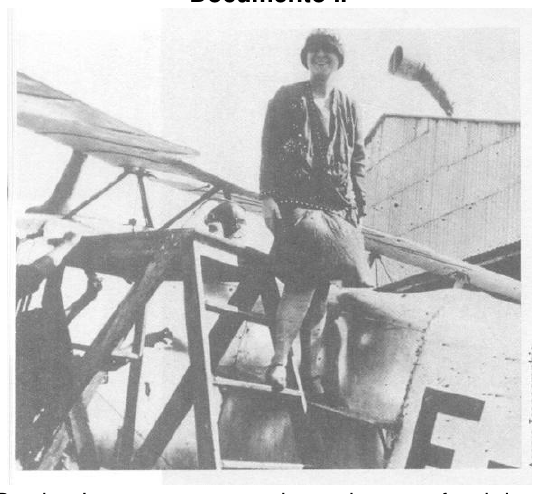
\includegraphics[width=0.95\linewidth]{static/simulados/coluni/figuras/2020/questao-35/figura-2.png}
\end{figure}
% COLUNI-AUTO-FIGURES-END

Bertha Lutz em campanha pelo voto feminino, c. 1928.

BOULOS JÚNIOR, Alfredo. \textbf{História sociedade \& Cidadania}, 9º ano. 3. ed. São Paulo: FTD, 2015, p. 142.

\textbf{Documento III}

% COLUNI-AUTO-FIGURES-BEGIN
\begin{figure}[htbp]
\centering
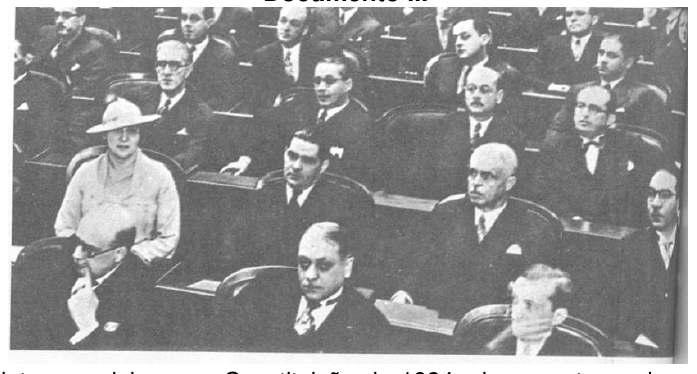
\includegraphics[width=0.95\linewidth]{static/simulados/coluni/figuras/2020/questao-35/figura-3.png}
\end{figure}
% COLUNI-AUTO-FIGURES-END

Na Assembleia Constituinte que elaborou a Constituição de 1934, via-se, entre os homens, uma única mulher. Seu nome era Carlota Pereira de Queirós. Foi ela a primeira mulher a ocupar o cargo de deputada no Brasil.

BOULOS JÚNIOR, Alfredo. \textbf{História sociedade \& Cidadania}, 9º ano. 3. ed. São Paulo: FTD, 2015, p. 142.

Sobre o reconhecimento do direito ao voto feminino no século XX, é INCORRETO afirmar que:
\begin{enumerate}
\item foi precedido por manifestações de diversas mulheres, grupos e associações sufragistas que se
        organizaram na luta pelo direito à participação política nos continentes europeu e americano.
\item foi uma concessão assegurada pelo decreto-lei assinado por Getúlio Vargas, em 1932, posteriormente
        incorporado à Constituição de 1934, a qual previa a obrigatoriedade do voto feminino.
\item foi influenciado pela ação de Bertha Lutz, liderança feminista brasileira que, inspirada no movimento
        sufragista europeu, empenhou-se na campanha pelos direitos femininos ao voto e à candidatura no Brasil.
\item foi marcado pela participação de Carlota Pereira de Queirós, primeira mulher a ocupar o cargo de
        deputada no Brasil, tendo participado da Assembleia Constituinte que elaborou a Constituição de 1934.
\end{enumerate}
